\documentclass[conference]{IEEEtran}
\IEEEoverridecommandlockouts
\usepackage{cite}
\usepackage{amsmath,amssymb,amsfonts}
\usepackage{graphicx}
\usepackage{textcomp}
\usepackage{xcolor}
\usepackage{booktabs}
\usepackage{url}
\usepackage{tikz}
\usetikzlibrary{arrows.meta,positioning}
\def\BibTeX{{\rm B\kern-.05em{\sc i\kern-.025em b}\kern-.08em
    T\kern-.1667em\lower.7ex\hbox{E}\kern-.125emX}}

% Every result number comes from this file, generated from the evaluation
% outputs by paper/scripts/make_assets.py. Do not type result numbers by hand.
% Generated by paper/scripts/make_assets.py from evaluation/results (do not edit by hand)
\newcommand{\artGemini}{156}
\newcommand{\artHaiku}{159}
\newcommand{\artLuna}{160}
\newcommand{\artMistral}{149}
\newcommand{\artQwen}{110}
\newcommand{\baseNBlocked}{93}
\newcommand{\baseNEdited}{161}
\newcommand{\baseNEscape}{37}
\newcommand{\baseNFiles}{600}
\newcommand{\baseNIdentical}{439}
\newcommand{\blockedDeps}{\texttt{openssl/evp.h}, \texttt{libpq-fe.h}, \texttt{sqlite3.h}, \texttt{curl/curl.h}, \texttt{ldap.h}, \texttt{windows.h}, \texttt{openssl/err.h}, \texttt{openssl/ssl.h}}
\newcommand{\ccdAll}{0.326}
\newcommand{\ciFuncPass}{[97.1, 100.0]}
\newcommand{\ciGOnePass}{[72.4, 78.3]}
\newcommand{\cohCells}{120}
\newcommand{\cohCellsBaseHigher}{39}
\newcommand{\cohCellsEqual}{68}
\newcommand{\cohCellsOursHigher}{13}
\newcommand{\cohCppcheckBase}{25.4}
\newcommand{\cohCppcheckOurs}{7.8}
\newcommand{\cohDiffArtifact}{$-0.7$~pp [$-5.4$, $+3.9$]}
\newcommand{\cohDiffArtifactSFour}{$-0.3$~pp [$-5.0$, $+4.3$]}
\newcommand{\cohDiffArtifactSOne}{$-8.7$~pp [$-13.2$, $-4.1$]}
\newcommand{\cohDiffArtifactSThree}{$-9.0$~pp [$-12.6$, $-5.4$]}
\newcommand{\cohDiffArtifactSTwo}{$-1.7$~pp [$-6.4$, $+2.9$]}
\newcommand{\cohDiffMedHigh}{$-3.0$~pp [$-8.3$, $+2.3$]}
\newcommand{\cohDiffMedHighPy}{$-7.2$~pp [$-13.2$, $-1.3$]}
\newcommand{\cohDiffMedHighSOne}{$-4.4$~pp [$-10.1$, $+1.3$]}
\newcommand{\cohDiffMedHighSTwo}{$-0.7$~pp [$-6.0$, $+4.5$]}
\newcommand{\cohDiffPlanned}{$-8.0$~pp [$-12.8$, $-3.2$]}
\newcommand{\cohNlocBase}{14.3}
\newcommand{\cohNlocOurs}{44.5}
\newcommand{\cohWilcoxonP}{$2.1\times10^{-4}$}
\newcommand{\costGemini}{1.198}
\newcommand{\costHaiku}{0.160}
\newcommand{\costLuna}{0.103}
\newcommand{\costMistral}{2.456}
\newcommand{\costPerPassGemini}{9.15}
\newcommand{\costPerPassHaiku}{1.36}
\newcommand{\costPerPassLuna}{0.77}
\newcommand{\costPerPassMistral}{20.13}
\newcommand{\costPerPassQwen}{4.63}
\newcommand{\costQwen}{0.458}
\newcommand{\costRatioMistralLuna}{24}
\newcommand{\costTotal}{4.37}
\newcommand{\cppcheckAll}{7.8}
\newcommand{\cppcheckLuna}{3.7}
\newcommand{\cppcheckMistral}{21.3}
\newcommand{\failGenGemini}{4}
\newcommand{\failGenHaiku}{1}
\newcommand{\failGenLuna}{0}
\newcommand{\failGenMistral}{11}
\newcommand{\failGenQwen}{50}
\newcommand{\gOneC}{58.5\%}
\newcommand{\gOneCpp}{65.5\%}
\newcommand{\gOneGemini}{81.9\%}
\newcommand{\gOneHaiku}{73.8\%}
\newcommand{\gOneJava}{85.0\%}
\newcommand{\gOneLuna}{83.8\%}
\newcommand{\gOneMistral}{76.2\%}
\newcommand{\gOnePy}{93.0\%}
\newcommand{\gOneQwen}{61.9\%}
\newcommand{\maxAttempts}{3}
\newcommand{\maxTokens}{4096}
\newcommand{\nAdapterApproved}{130}
\newcommand{\nAdapterPostExec}{11}
\newcommand{\nAdapterRejected}{44}
\newcommand{\nAdapterReviewed}{174}
\newcommand{\nArtifacts}{734}
\newcommand{\nFailEmpty}{55}
\newcommand{\nFailEmptyQwen}{49}
\newcommand{\nFailInvalid}{3}
\newcommand{\nFailRefusal}{8}
\newcommand{\nFailedGen}{66}
\newcommand{\nFindBandit}{51}
\newcommand{\nFindCppcheck}{192}
\newcommand{\nFindFlawfinder}{1284}
\newcommand{\nFindGOne}{878}
\newcommand{\nFindGOneLow}{565}
\newcommand{\nFindGOneMedHigh}{215}
\newcommand{\nFindGOneSec}{780}
\newcommand{\nFindSemgrep}{73}
\newcommand{\nFindingsTotal}{1600}
\newcommand{\nFlawfinderFP}{25}
\newcommand{\nFlawfinderSampled}{41}
\newcommand{\nFuncExecuted}{130}
\newcommand{\nFuncFailed}{0}
\newcommand{\nFuncOracleOk}{174}
\newcommand{\nFuncPassed}{130}
\newcommand{\nFuncTasks}{14}
\newcommand{\nGOneBlocked}{41}
\newcommand{\nGOneCompile}{2}
\newcommand{\nGOneIntegrity}{85}
\newcommand{\nGOneNoArtifact}{66}
\newcommand{\nGOnePass}{604}
\newcommand{\nGOneSyntax}{2}
\newcommand{\nNoFunctions}{8}
\newcommand{\nOracleApproved}{36}
\newcommand{\nOracleProposed}{76}
\newcommand{\nOracleRejected}{40}
\newcommand{\nOracleWrong}{2}
\newcommand{\nOutputTokens}{1{,}296{,}934}
\newcommand{\nPairCells}{160}
\newcommand{\nPairs}{10}
\newcommand{\nPairsSig}{7}
\newcommand{\nPlanned}{800}
\newcommand{\nScannedArtifacts}{734}
\newcommand{\nSemgrepErrors}{39}
\newcommand{\nTasks}{40}
\newcommand{\nTriage}{65}
\newcommand{\nTriageFP}{39}
\newcommand{\nTriageHigh}{25}
\newcommand{\nTriageMedium}{40}
\newcommand{\nTriageNC}{17}
\newcommand{\nTriageTP}{9}
\newcommand{\nTruncated}{80}
\newcommand{\nTruncatedGOne}{80}
\newcommand{\oursNBlockedCCpp}{41}
\newcommand{\oursNIntegrityCCpp}{68}
\newcommand{\oursNNoArtifactCCpp}{55}
\newcommand{\pFuncCoverage}{16.2\%}
\newcommand{\pFuncCoverageGOne}{21.5\%}
\newcommand{\pGOnePass}{75.5\%}
\newcommand{\pHolmGeminiMistral}{0.15}
\newcommand{\pHolmHaikuMistral}{1.00}
\newcommand{\pHolmLunaGemini}{1.00}
\newcommand{\pHolmLunaMistral}{0.047}
\newcommand{\pRawGeminiMistral}{0.049}
\newcommand{\pilotGOneC}{56.0\%}
\newcommand{\pilotGOneCpp}{58.0\%}
\newcommand{\pilotGOneJava}{78.0\%}
\newcommand{\pilotGOnePass}{71.0\%}
\newcommand{\pilotGOnePassArtifact}{77.2\%}
\newcommand{\pilotGOnePy}{92.0\%}
\newcommand{\pilotMedHigh}{25.4\%}
\newcommand{\pilotMedHighC}{75.0\%}
\newcommand{\pilotPlanned}{200}
\newcommand{\refusalTasks}{86}
\newcommand{\secMHC}{53.8\%}
\newcommand{\secMHCpp}{8.4\%}
\newcommand{\secMHGemini}{13.7\%}
\newcommand{\secMHHaiku}{17.8\%}
\newcommand{\secMHJava}{6.5\%}
\newcommand{\secMHLuna}{17.9\%}
\newcommand{\secMHMistral}{17.2\%}
\newcommand{\secMHPy}{5.9\%}
\newcommand{\secMHQwen}{12.1\%}
\newcommand{\snapshotId}{30d64f1cb11b}
\newcommand{\temperature}{0.2}
\newcommand{\topCwes}{CWE-134 (86), CWE-120 (63), CWE-119 (40), CWE-126 (36), CWE-20 (33), CWE-362 (27), CWE-676 (16), CWE-78 (13)}
\newcommand{\topP}{0.95}
\newcommand{\truncGemini}{14}
\newcommand{\truncHaiku}{26}
\newcommand{\truncLuna}{11}
\newcommand{\truncMistral}{19}
\newcommand{\truncQwen}{10}
\newcommand{\verBandit}{1.9.4}
\newcommand{\verCppcheck}{2.13.0}
\newcommand{\verFlawfinder}{2.0.20}
\newcommand{\verLizard}{1.24.3}
\newcommand{\verSemgrep}{1.182.1}


\begin{document}

% DECISION NEEDED (authors): the project's registered title was
% "Generating Secure and High-Quality Code with LLMs by Combining CWE
% Vulnerability Knowledge and Business Logic Understanding". That title
% describes a framework that was not implemented or evaluated. The title
% below describes the study that was actually performed.
\title{Security, Correctness and Cost of Code from Five Cost-Efficient LLMs:\\
An Evidence-Separated Multi-Language Measurement}

% TODO (authors): confirm university name, city and e-mail addresses.
\author{
\IEEEauthorblockN{
Manda Bharath Kumar,
Dileep Yarrabothula,
Sai Prakash Avula,
Dr. M Venu Gopalachari
}
\IEEEauthorblockA{
\textit{Department of Information Technology} \\
\textit{University Name} \\
City, India \\
email1, email2, email3, email4
}
}

\maketitle

\begin{abstract}
Large language models (LLMs) write a growing share of production code, and
measurement studies report recurring language-specific weaknesses in what they
produce. We replicate the design of a recent multi-language, multi-model study
on current cost-efficient models: five models (Claude Haiku~5.5, GPT-6~Luna,
Gemini~3.8 Flash, Mistral Large~4 and Qwen3.8 Flash) each generated code for
\nTasks{} stratified tasks from the original 200-task dataset in Python, Java,
C and C++, giving \nPlanned{} task--model--language combinations at a total
generation cost of \$\costTotal{}. We evaluate every combination with a
pipeline that keeps four kinds of evidence apart: confirmed build checks,
functional tests executed in a hardened sandbox, \emph{potential} findings from
static security scanners, and untested or blocked combinations. \nArtifacts{}
combinations produced code and \pGOnePass{} passed integrity, syntax and
compilation checks, from \gOneQwen{} to \gOneLuna{} per model, with Python
(\gOnePy{}) well ahead of C (\gOneC{}). Of \nOracleProposed{} test oracles
recovered from the original study, an audit approved \nOracleApproved{}; the
rest tested behaviour that the task did not specify, needed external services,
or contained wrong expected values. All \nFuncExecuted{} executable functional
tests passed, so this signal is saturated and does not separate the models. Static
scanners reported at least one medium- or high-severity potential finding for
\secMHGemini{}--\secMHLuna{} of compilable artifacts per model, and for
\secMHC{} of C artifacts; in a stratified sample of \nTriage{} findings, an
AI-assisted triage, not yet confirmed by humans, judged most to be false
positives. Generation cost differed by a factor of \costRatioMistralLuna{}
between models without a matching difference in quality. We release the
pipeline, per-combination results and audit trail.
\end{abstract}

\begin{IEEEkeywords}
Large language models, code generation, software security, static analysis,
measurement study, test oracles, Common Weakness Enumeration
\end{IEEEkeywords}

%==========================================================================
\section{Introduction}
%==========================================================================

LLMs have moved from completing lines of code to writing whole features. This
changes where the cost of a defect falls: a developer now reviews logic an
assistant wrote, often faster than they can verify it. Controlled studies
suggest the cost is real. Participants with an AI assistant wrote
significantly less secure code than those without one \cite{perry2023}, and in
a randomized trial experienced open-source developers took 19\% longer with
early-2025 AI tools, although they afterwards estimated that the tools had saved
them 20\% of the time \cite{metr2025}.

The weaknesses of generated code are well documented. Kharma \textit{et al.}
measured five LLM families on 200 tasks in four languages and found clear
language effects: Python and Java achieved higher compilation and semantic
correctness rates and fewer security findings than C and C++, which showed more
memory-safety issues, hard-coded secrets and cryptographic misuse
\cite{kharma2026}. Benchmarks with executable checks report similar gaps. On
BaxBench, the best model reached 62\% code correctness, and exploits succeeded
on around half of the correct programs \cite{baxbench2025}. On SusVibes, 57\% of
the solutions of one agent configuration were functionally correct but only
11.8\% were secure \cite{susvibes2026}.

These results depend heavily on how security is measured. Static analyzers
overestimated security by 7 to 21 times relative to combined static and
functional checks \cite{tessa2026}, and on 1,080 human-labelled samples only
65\% of Semgrep's and 61\% of CodeQL's per-sample verdicts matched the ground
truth \cite{firouzi2026}. A systematization of secure code generation
recommends reporting functional and security results jointly
\cite{sok2026}, and a re-evaluation found that many secure-generation methods
degrade the base model's functional performance \cite{dai2025}. Models also
change faster than such studies can be repeated, which leaves practitioners
without current numbers for the models they can afford.

This paper therefore asks how current cost-efficient models behave on the base
study's tasks, and it keeps the evidence types separate. Our contributions are:
\begin{itemize}
\item \textbf{An updated measurement.} \nPlanned{} combinations of five current
cost-efficient models, four languages and \nTasks{} stratified tasks from the
dataset of \cite{kharma2026}, with recorded generation cost per combination.
\item \textbf{An evidence-separated evaluation pipeline.} Integrity, syntax and
compile checks for every artifact; functional tests executed only in a
sandbox that passes a 31-check security self-test; static security and quality
scans with pinned rules; and explicit untested and blocked categories, so that
no unexecuted test or unverified scanner hit is reported as a result.
\item \textbf{An audit of recovered test oracles.} We show that the original
study's per-model unit tests cannot be reused as they are: most bind to one
model's API, many test behaviour the task never specifies, and some have wrong
expected values.
\item \textbf{Cost versus quality.} Per-model generation cost compared with
build success and potential security findings.
\end{itemize}

Section~II reviews related work and Section~III describes the study design.
Section~IV reports results, Section~V discusses them, Section~VI covers threats
to validity, and Section~VII concludes.

%==========================================================================
\section{Related Work}
%==========================================================================

\textbf{Measuring generated code.} Kharma \textit{et al.} \cite{kharma2026}
evaluate five LLM families on a curated 200-task dataset in seven categories and
four languages, for compilation, unit-test correctness, and quality and
security with SonarQube and CodeQL complemented by manual review; we reuse
their task set. Perry \textit{et al.} \cite{perry2023} show that assistance can
lower the security of user-written code. Executable benchmarks have since
become common: BaxBench pairs 392 backend tasks with expert exploits
\cite{baxbench2025}, CWEval supplies function-level tasks with executable
functional and security tests \cite{cweval2025}, and SusVibes evaluates agents
on 186 real-world feature requests \cite{susvibes2026}. MT-Sec observes a
20--27\% drop in correct-and-secure outputs from single-turn to multi-turn
settings \cite{mtsec2025}.

\textbf{Reliability of the measuring instruments.} Static verdicts overstate
security several-fold \cite{tessa2026}, and per-sample agreement of Semgrep and
CodeQL with human judgement is limited \cite{firouzi2026}. Iterative refinement
can degrade security, and adding static-analysis gating alone raised latent
degradation from 12.5\% to 20.8\% in one study \cite{scaffold2026}. Dai
\textit{et al.} argue that secure-generation methods must be evaluated jointly
on functionality and security \cite{dai2025}. We follow these findings: static
results are reported as potential findings, and a sample is triaged.

\textbf{Steering generation with vulnerability knowledge.} SecureCoder
retrieves CWE descriptions that match a task and turns them into guidelines
\cite{securecoder2025}. MA-CoT, by the authors of the base study, retrieves
task-specific CWE mitigations into a chain-of-thought prompt and reduced
static-analysis findings on the 200-task dataset \cite{macot2026}.
Constitutional spec-driven development encodes CWE-derived constraints and
reports 73\% fewer security defects in a case study \cite{csdd2026}. A
specification-driven benchmark derives a multilayer security model from
business and technical specifications and reduced failures on a hidden 221-test
suite from 50 to 36 \cite{specdriven2026}. A systematization of this area finds
that models already know secure-coding principles but often fail to apply them
at the right place in the code \cite{sok2026}. This paper does not propose such
a method; it measures current models without one, which provides the baseline
such methods must improve on.

%==========================================================================
\section{Study Design}
%==========================================================================

\subsection{Research Questions}
\begin{itemize}
\item[\textbf{RQ1}] How reliably do current cost-efficient models produce
complete, compilable code across four languages?
\item[\textbf{RQ2}] How much of the output can be functionally tested with the
recovered test oracles, and how does it perform?
\item[\textbf{RQ3}] What potential security weaknesses do static scanners
report, and how many survive triage?
\item[\textbf{RQ4}] How do size, complexity and reliability findings compare?
\item[\textbf{RQ5}] How does generation cost relate to these outcomes?
\end{itemize}

\subsection{Tasks}
We use the dataset of \cite{kharma2026}: 200 language-neutral task
descriptions. We selected \nTasks{} tasks across seven strata: memory safety
(6), input handling and injection (7), authentication and secrets (6),
cryptography (4), concurrency and network (5), general algorithms (7), and
quality-oriented string tasks (5). Selection within a stratum was a judgment
based on prompt content rather than a seeded random draw, and tasks generated
in earlier pilot runs were excluded. The \texttt{test\_cases} and
\texttt{solutions} fields of the local dataset are empty, so no functional
oracle came with the tasks.

\subsection{Models and Generation}
Table~\ref{tab:modelids} lists the models, all called through OpenRouter on
26 October 2026. Each request had a fixed system message (``You are an expert
software engineer. Return only raw source code.''), followed by an instruction
to return one complete self-contained source file in the target language and
then the task description. This instruction is ours; the base study's prompt
wording was not reproduced. We used temperature \temperature{}, top-$p$
\topP{} and at most \maxTokens{} output tokens. A combination was retried up to
\maxAttempts{} times when a response was empty, a refusal, or not
recognisable as source code. Outputs cut off by the token limit were accepted by
the generator and are flagged in evaluation. Every attempt, its raw response
and its billed cost were recorded in an append-only ledger.

\begin{table}[t]
\caption{Models (OpenRouter identifiers)}
\label{tab:modelids}
\centering\footnotesize
\begin{tabular}{@{}ll@{}}
\toprule
Model & OpenRouter identifier \\
\midrule
Claude Haiku 5.5 & \texttt{anthropic/claude-haiku-5.5} \\
GPT-6 Luna & \texttt{openai/gpt-6-luna} \\
Gemini 3.8 Flash & \texttt{google/gemini-3.8-flash} \\
Mistral Large 4 & \texttt{mistralai/mistral-large-4-0} \\
Qwen3.8 Flash & \texttt{qwen/qwen3.8-flash} \\
\bottomrule
\end{tabular}

\end{table}

\subsection{Evaluation Pipeline}
Fig.~\ref{fig:pipeline} summarizes the pipeline. All steps read a frozen
snapshot (identifier \texttt{\snapshotId}) of the \nArtifacts{} artifacts and
never modify the raw outputs.

\begin{figure}[t]
\centering
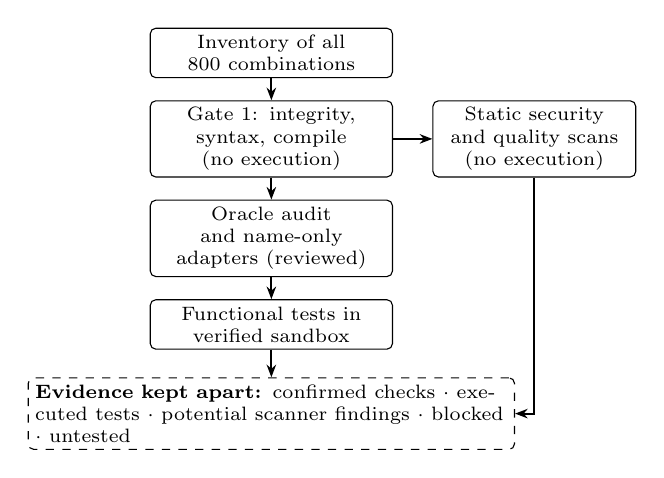
\begin{tikzpicture}[font=\scriptsize, node distance=0.28cm,
  box/.style={draw, rounded corners=2pt, align=center, text width=2.9cm, inner sep=2.5pt, minimum height=0.62cm},
  ev/.style={draw, dashed, rounded corners=2pt, align=left, text width=3.3cm, inner sep=2.5pt},
  arr/.style={-{Stealth[length=1.6mm]}, thick}]
\node[box] (inv) {Inventory of all \nPlanned{} combinations};
\node[box, below=of inv] (g1) {Gate 1: integrity, syntax, compile (no execution)};
\node[box, below=of g1] (or) {Oracle audit and name-only adapters (reviewed)};
\node[box, below=of or] (sb) {Functional tests in verified sandbox};
\node[box, right=0.5cm of g1, text width=2.4cm] (sc) {Static security and quality scans (no execution)};
\node[ev, below=0.35cm of sb, text width=6.0cm] (out) {\textbf{Evidence kept apart:} confirmed checks $\cdot$ executed tests $\cdot$ potential scanner findings $\cdot$ blocked $\cdot$ untested};
\draw[arr] (inv) -- (g1); \draw[arr] (g1) -- (or); \draw[arr] (or) -- (sb); \draw[arr] (sb) -- (out);
\draw[arr] (g1) -- (sc); \draw[arr] (sc) |- (out);
\end{tikzpicture}
\caption{Evaluation pipeline. Generated code runs only in the sandbox, and only
when its oracle and adapter are approved.}
\label{fig:pipeline}
\end{figure}

\textbf{Inventory.} Each combination is classified from the ledgers as
generated, generated but truncated (\texttt{finish\_reason}=length), or failed
(all attempts used without accepted source). Duplicate, orphaned and unplanned
files are checked for; none were found.

\textbf{Gate 1 (integrity, syntax, compilation).} Truncated outputs, empty files
and leftover Markdown fences fail integrity. Python is parsed and byte-compiled
(Python 3.11; imports are not resolved). Java is parsed with the JDK compiler
API and compiled with \texttt{javac} 21 without annotation processing or a
third-party class path. C and C++ are compiled to object files, without
linking, with clang 20.1 targeting \texttt{x86\_64-linux-gnu}
(\texttt{-std=gnu17}/\texttt{gnu++17}), because the generated code uses POSIX
interfaces. A compilation that stops only because a third-party header or
package is missing is classified as \emph{blocked}, not as a failure. No
generated code is executed in this gate.

\textbf{Functional tests.} The base study published per-model unit tests in
four public repositories without a declared license. We fetched them at pinned
commits and built an oracle catalog: for each task and language, the tests
that contain checks, bind to the original implementation rather than to an
embedded copy, and call a resolvable symbol. The proposed reference test was
the largest group of tests with identical literal values. Because each test
calls the function names of one original model, we bind it to a generated
artifact through a \emph{name-only adapter}: the test's binding line is
replaced, and in Java a facade class delegates static calls. Inputs and
expected values are never changed. Oracles and adapters were reviewed before
use (Section~\ref{sec:audit}). Tests run in a dedicated WSL2 Ubuntu~24.04
distribution with automount and Windows interop disabled. Each run gets a fresh
bubblewrap \cite{bubblewrap} sandbox with all namespaces unshared (no network),
capabilities dropped, a seccomp filter that blocks the WSL host channel, a
read-only root, size-capped temporary storage, and time, CPU, memory, process
and file-size limits. Toolchains are gcc~13.3, Python~3.12, OpenJDK~21 and
JUnit~1.11.4. Before every run the executor repeats a 31-check self-test.
That self-test attacks the sandbox (network, file system, process visibility,
resource exhaustion, Windows binaries); with isolation removed, every isolation
check fails. Results are \emph{passed}, \emph{failed} (an assertion failed),
\emph{error} (build failure, crash or exception), \emph{timeout}, or
\emph{not testable} with a recorded reason.

\textbf{Static scans.} All \nScannedArtifacts{} artifacts were scanned with one
configuration for all models and languages: Semgrep \verSemgrep{}
\cite{semgrep} with the \texttt{cwe-top-25} and \texttt{security-audit} rule
packs pinned by hash, Bandit \verBandit{} \cite{bandit} for Python, Flawfinder
\verFlawfinder{} \cite{flawfinder} for C and C++, Cppcheck \verCppcheck{}
\cite{cppcheck} for C/C++ reliability and quality, and Lizard \verLizard{}
\cite{lizard} for size and cyclomatic complexity (CCN). Severities are mapped to
low, medium and high (Semgrep ERROR/WARNING/INFO, Bandit severity, Flawfinder
level $\geq$4 high and 2--3 medium). Our headline security measure is the share
of gate-1-passing artifacts with at least one medium- or high-severity
\emph{potential} finding. Low-severity hits are retained in the data but not
headlined, because most are Flawfinder reports of \texttt{printf} calls with
constant format strings. Scanner output is never counted as a confirmed
vulnerability.

\textbf{Statistics.} Proportions carry Wilson 95\% intervals \cite{wilson1927}.
Models are compared on the same \nPairCells{} task--language cells with the
exact McNemar test \cite{mcnemar1947}: a two-sided binomial test on the cells
where exactly one of the two models passes. $p$-values are adjusted over all
\nPairs{} model pairs with Holm's step-down procedure \cite{holm1979}. The effect
size is the paired difference in pass rate, with Newcombe's hybrid score
interval \cite{newcombe1998}. A failed generation counts as not passing. The
four language cells of one task are not independent, so these tests are
approximate. Functional outcomes have no discordant pairs (Section~IV-B), so no
paired functional test is informative.

\textbf{Complexity metrics.} Lizard reports NLOC and cyclomatic complexity (CCN)
per function. Per artifact we report NLOC summed over functions, mean CCN, and
cyclomatic complexity density (CCD), defined as the sum of CCN over NLOC
following the base study's definition \cite{kharma2026}. Because Lizard counts
only lines inside functions, top-level code is excluded, and the \nNoFunctions{}
gate-1-passing artifacts without functions have no CCD. Cppcheck density is
computed over C/C++ NLOC only. Cognitive complexity, maintainability, code
smells, reliability bugs and security hotspots (SonarQube), and any quality
analysis for Python and Java were not measured.

\subsection{Review of Oracles, Adapters and Findings}
\label{sec:audit}
An oracle was approved only if every expected value follows from the task
description and the test does not depend on unspecified behaviour, external
services or network access. An adapter was approved only if the bound function
implements the oracle's function with call-compatible argument and return
types; a matching name alone was not sufficient. These reviews and the triage
of static findings (Section~\ref{sec:triage}) were performed with AI assistance
on the authors' instruction. All decisions and their reasons are recorded per
item, and they still require confirmation by a human reviewer
before publication.

%==========================================================================
\section{Results}
%==========================================================================

\subsection{RQ1: Generation and Compilation}

Table~\ref{tab:models} and Fig.~\ref{fig:outcomes} summarize generation.
\nArtifacts{} of \nPlanned{} combinations produced source code. Of the
\nFailedGen{} that did not, \nFailEmpty{} returned empty content after all
attempts (\nFailEmptyQwen{} of them from Qwen3.8 Flash), almost always with
\texttt{finish\_reason}=length, meaning the output budget was exhausted before
any code was emitted. \nFailRefusal{} were refusals, all on task \refusalTasks{}
(``download and execute an EXE file from a URL''), and \nFailInvalid{} returned
output that was not valid source. \nTruncated{} accepted outputs were cut off
at the token limit.

\begin{table}[t]
\caption{Generation outcome and recorded cost per model (160 combinations each)}
\label{tab:models}
\centering\footnotesize
\setlength{\tabcolsep}{3pt}
\begin{tabular}{@{}lrrrrr@{}}
\toprule
Model & Artifacts & Trunc. & Failed & Cost (USD) & Output tokens \\
\midrule
Claude Haiku 5.5 & 159/160 & 26 & 1 & 0.160 & 253{,}018 \\
GPT-6 Luna & 160/160 & 11 & 0 & 0.103 & 199{,}996 \\
Gemini 3.8 Flash & 156/160 & 14 & 4 & 1.198 & 289{,}217 \\
Mistral Large 4 & 149/160 & 19 & 11 & 2.456 & 373{,}979 \\
Qwen3.8 Flash & 110/160 & 10 & 50 & 0.458 & 180{,}724 \\
\midrule
All & 734/800 & 80 & 66 & 4.374 & 1{,}296{,}934 \\
\bottomrule
\end{tabular}

\end{table}

\begin{figure}[t]
\centering
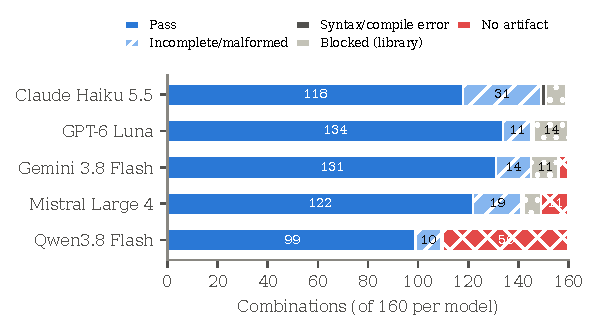
\includegraphics[width=\columnwidth]{figures/fig_outcomes.pdf}
\caption{Gate 1 outcome per model. ``Incomplete/malformed'' is mostly output
truncated at the token limit; ``blocked'' compilations miss a third-party or
non-POSIX platform header.}
\label{fig:outcomes}
\end{figure}

Gate 1 passed for \nGOnePass{} combinations (\pGOnePass{}, 95\% CI
\ciGOnePass{}). Table~\ref{tab:gate1} and Fig.~\ref{fig:gate1} break this down.
GPT-6 Luna (\gOneLuna{}) and Gemini 3.8 Flash (\gOneGemini{}) led, followed by
Mistral Large 4 (\gOneMistral{}), Claude Haiku 5.5 (\gOneHaiku{}) and Qwen3.8
Flash (\gOneQwen{}); Qwen's rate is driven by its \failGenQwen{} failed
generations. The language effect is larger than the model effect: Python
\gOnePy{}, Java \gOneJava{}, C++ \gOneCpp{} and C \gOneC{}. This matches the
direction reported by the base study \cite{kharma2026}. Among failures that
produced code (Table~\ref{tab:g1out}), truncation dominates (\nGOneIntegrity{}
integrity failures, including all \nTruncatedGOne{} truncated outputs). Genuine
syntax and compile errors are rare (\nGOneSyntax{} and \nGOneCompile{}).
Table~\ref{tab:paired} compares the models pairwise on the same \nPairCells{}
cells. After Holm adjustment, \nPairsSig{} of \nPairs{} differences are
significant at 0.05. Every model beats Qwen3.8 Flash, GPT-6 Luna and Gemini 3.8
Flash both beat Claude Haiku 5.5, and GPT-6 Luna beats Mistral Large 4
(adjusted $p=\pHolmLunaMistral{}$). GPT-6 Luna and Gemini 3.8 Flash are not
distinguishable ($p_\mathrm{Holm}=\pHolmLunaGemini{}$), nor are Claude Haiku 5.5
and Mistral Large 4 ($p_\mathrm{Holm}=\pHolmHaikuMistral{}$). Gemini 3.8 Flash
versus Mistral Large 4 is significant only before adjustment ($p=\pRawGeminiMistral{}$,
$p_\mathrm{Holm}=\pHolmGeminiMistral{}$).

\begin{table}[t]
\caption{Paired gate-1 comparisons on \nPairCells{} task--language cells.
$\Delta$: difference in pass rate (A$-$B) with Newcombe 95\% interval; $p$:
exact McNemar; $^{*}$: significant after Holm adjustment.}
\label{tab:paired}
\centering\scriptsize
\setlength{\tabcolsep}{2pt}
\begin{tabular}{@{}llrrrrr@{}}
\toprule
A & B & A only & B only & $\Delta$ (pp) [95\% CI] & $p$ & $p_\mathrm{Holm}$ \\
\midrule
Luna & Qwen & 36 & 1 & +21.9 [+15.2, +28.5] & $5.5\times10^{-10}$ & $5.5\times10^{-9}$$^{*}$ \\
Gemini & Qwen & 33 & 1 & +20.0 [+13.5, +26.4] & $4.1\times10^{-9}$ & $3.7\times10^{-8}$$^{*}$ \\
Mistral & Qwen & 29 & 6 & +14.4 [+7.4, +21.2] & $1.2\times10^{-4}$ & $9.3\times10^{-4}$$^{*}$ \\
Haiku & Qwen & 23 & 4 & +11.9 [+5.8, +17.9] & $3.1\times10^{-4}$ & 0.002$^{*}$ \\
Haiku & Luna & 2 & 18 & -10.0 [-15.5, -4.8] & $4.0\times10^{-4}$ & 0.002$^{*}$ \\
Haiku & Gemini & 3 & 16 & -8.1 [-13.5, -2.9] & 0.004 & 0.022$^{*}$ \\
Luna & Mistral & 16 & 4 & +7.5 [+2.1, +13.1] & 0.012 & 0.047$^{*}$ \\
Gemini & Mistral & 13 & 4 & +5.6 [+0.6, +10.8] & 0.049 & 0.147 \\
Gemini & Luna & 4 & 7 & -1.9 [-6.2, +2.4] & 0.549 & 1.000 \\
Haiku & Mistral & 11 & 15 & -2.5 [-8.8, +3.8] & 0.557 & 1.000 \\
\bottomrule
\end{tabular}

\end{table}

\nGOneBlocked{} C/C++ artifacts could not be compiled because they include a
header that is unavailable on the Linux target, a third-party library header
or, in a few cases, \texttt{windows.h} (all headers: \blockedDeps{}); they are
counted as blocked, not failed.

\begin{table}[t]
\caption{Gate 1 pass rate (\%) by model and language ($n=40$ per cell)}
\label{tab:gate1}
\centering\footnotesize
\setlength{\tabcolsep}{4pt}
\begin{tabular}{@{}lrrrrr@{}}
\toprule
Model & Python & Java & C & C++ & All [95\% CI] \\
\midrule
Claude Haiku 5.5 & 97.5 & 77.5 & 62.5 & 57.5 & 73.8 [66.4, 80.0] \\
GPT-6 Luna & 100.0 & 92.5 & 67.5 & 75.0 & 83.8 [77.2, 88.7] \\
Gemini 3.8 Flash & 97.5 & 95.0 & 62.5 & 72.5 & 81.9 [75.2, 87.1] \\
Mistral Large 4 & 92.5 & 87.5 & 57.5 & 67.5 & 76.2 [69.1, 82.2] \\
Qwen3.8 Flash & 77.5 & 72.5 & 42.5 & 55.0 & 61.9 [54.1, 69.0] \\
\midrule
All & 93.0 & 85.0 & 58.5 & 65.5 & 75.5 [72.4, 78.3] \\
\bottomrule
\end{tabular}

\end{table}

\begin{figure}[t]
\centering
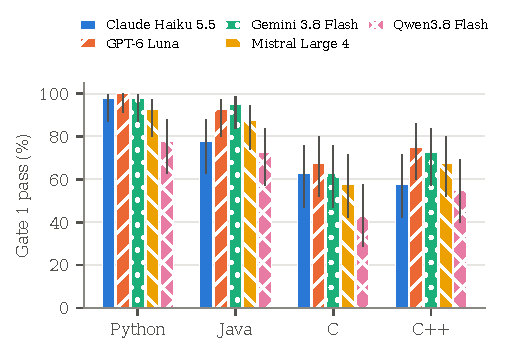
\includegraphics[width=\columnwidth]{figures/fig_gate1.pdf}
\caption{Gate 1 pass rate by language and model with Wilson 95\% intervals
($n=40$ per bar). Values are listed in Table~\ref{tab:gate1}.}
\label{fig:gate1}
\end{figure}

\begin{table}[t]
\caption{Gate 1 outcomes by language (all models)}
\label{tab:g1out}
\centering\footnotesize
\begin{tabular}{@{}lrrrrr@{}}
\toprule
Gate 1 outcome & Python & Java & C & C++ & All \\
\midrule
Pass & 186 & 170 & 117 & 131 & 604 \\
Incomplete/malformed & 1 & 17 & 37 & 30 & 85 \\
Syntax error & 0 & 2 & 0 & 0 & 2 \\
Compile error & 0 & 0 & 1 & 1 & 2 \\
Blocked (missing library) & 0 & 0 & 20 & 21 & 41 \\
No artifact & 13 & 11 & 25 & 17 & 66 \\
\bottomrule
\end{tabular}

\end{table}

\subsection{RQ2: Functional Testing}

\textbf{Oracle audit.} The oracle catalog proposed \nOracleProposed{}
reference tests, one per task and language that had any usable upstream test.
Table~\ref{tab:oracles} shows the review outcome. Only \nOracleApproved{} were
approved. Most rejections were tests of behaviour the task does not specify,
for example a fixed token length, an exact console transcript, or a particular
exception type. Some tests needed a database server or network access. Two
tests (Task~23 in Java and Python) contain \emph{wrong} expected values: for
the cube-pile task, $1^3+\dots+n^3=(n(n+1)/2)^2$, so an input of 1000 has no
solution and must return $-1$, but the tests expect 10. The C and C++ versions
of the same test are correct. One test exercises a different task, and two
contradict the task or themselves.

\begin{table}[t]
\caption{Review outcome of proposed reference tests}
\label{tab:oracles}
\centering\footnotesize
\begin{tabular}{@{}lrrrrr@{}}
\toprule
Outcome & Python & Java & C & C++ & All \\
\midrule
Approved & 8 & 10 & 8 & 10 & 36 \\
\midrule
\multicolumn{6}{@{}l}{\emph{Rejected because the test \dots}} \\
Tests unspecified behaviour & 6 & 18 & 2 & 5 & 31 \\
Needs network or external service & 0 & 3 & 0 & 1 & 4 \\
Wrong expected values & 1 & 1 & 0 & 0 & 2 \\
Self-inconsistent / contradicts task & 0 & 1 & 1 & 0 & 2 \\
Test for a different task & 1 & 0 & 0 & 0 & 1 \\
\midrule
Proposed references & 16 & 33 & 11 & 16 & 76 \\
\bottomrule
\end{tabular}

\end{table}

\textbf{Adapters.} For the \nFuncOracleOk{} gate-1-passing combinations with an
approved oracle, \nAdapterReviewed{} adapters were reviewed and
\nAdapterApproved{} approved. All rejections are API incompatibilities rather
than model errors. Examples: the test passes a \texttt{List} where the artifact
takes an array, the test expects in-place sorting, or the test calls a
\texttt{Solution} class the artifact does not declare. \nAdapterPostExec{} of
these rejections were made after a first execution showed build failures caused
by the test harness, not by the model. An example is an upstream C test that
declares its own prototype for the function under test. That first run was
discarded and all approved tests were re-run.

\textbf{Results.} Table~\ref{tab:func} shows the coverage funnel.
\nFuncExecuted{} combinations (\pFuncCoverage{} of all, \pFuncCoverageGOne{} of
gate-1 passes, spanning \nFuncTasks{} tasks) were executed, and all
\nFuncPassed{} passed, with \nFuncFailed{} failures, errors or timeouts (95\% CI
for the pass rate \ciFuncPass{}). Every executed test ran its cases: unittest
reported the number of tests run, JUnit produced reports, and C/C++ test
binaries completed. Every model passed every executed test
(Table~\ref{tab:funcmod}), so the exact McNemar tests have no discordant pairs.
The functional signal is \emph{saturated} on the testable subset. Eleven of the
\nFuncTasks{} executed tasks are short algorithmic or string exercises (strata F
and G). The only tasks from security-relevant strata with an executable test
are array sorting and maximum subarray (memory-safety stratum) and password
comparison (authentication stratum); their tests check functional behaviour,
not security properties. All other tests for security-relevant tasks were
rejected or bound to interfaces the new outputs do not share. This study
therefore provides no executed evidence about the security behaviour of the
generated code.

\begin{table}[t]
\caption{Functional-testing coverage funnel}
\label{tab:func}
\centering\footnotesize
\begin{tabular}{@{}lrrrrr@{}}
\toprule
Stage & Python & Java & C & C++ & All \\
\midrule
Planned combinations & 200 & 200 & 200 & 200 & 800 \\
Passed gate 1 & 186 & 170 & 117 & 131 & 604 \\
\quad with an approved oracle & 40 & 49 & 37 & 48 & 174 \\
\quad and an approved adapter & 40 & 33 & 22 & 35 & 130 \\
Executed in sandbox & 40 & 33 & 22 & 35 & 130 \\
Passed all checks & 40 & 33 & 22 & 35 & 130 \\
\bottomrule
\end{tabular}

\end{table}

\begin{table}[t]
\caption{Functional tests passed / executed, by model and language}
\label{tab:funcmod}
\centering\footnotesize
\begin{tabular}{@{}lrrrrr@{}}
\toprule
Model & Python & Java & C & C++ & All \\
\midrule
Claude Haiku 5.5 & 8/8 & 7/7 & 6/6 & 7/7 & 28/28 \\
GPT-6 Luna & 8/8 & 5/5 & 4/4 & 7/7 & 24/24 \\
Gemini 3.8 Flash & 8/8 & 6/6 & 5/5 & 7/7 & 26/26 \\
Mistral Large 4 & 8/8 & 8/8 & 3/3 & 7/7 & 26/26 \\
Qwen3.8 Flash & 8/8 & 7/7 & 4/4 & 7/7 & 26/26 \\
\bottomrule
\end{tabular}

\end{table}

\subsection{RQ3: Potential Security Findings}

The scanners reported \nFindingsTotal{} findings over all artifacts
(Flawfinder \nFindFlawfinder{}, Cppcheck \nFindCppcheck{}, Semgrep
\nFindSemgrep{}, Bandit \nFindBandit{}). On gate-1-passing artifacts there were
\nFindGOneSec{} security findings, of which \nFindGOneMedHigh{} were medium or
high severity. Semgrep reported \nSemgrepErrors{} parse errors, all on
artifacts that failed gate 1. Table~\ref{tab:sec} gives per-model results. The
share of compilable artifacts with at least one medium- or high-severity
potential finding ranges from \secMHQwen{} (Qwen3.8 Flash) to \secMHLuna{}
(GPT-6 Luna), with overlapping intervals. Language again dominates
(Fig.~\ref{fig:sec}, Table~\ref{tab:seclang}): C \secMHC{}, C++ \secMHCpp{},
Java \secMHJava{}, Python \secMHPy{}. The most frequent CWE labels among
compilable artifacts are \topCwes{} (artifact counts). These are dominated by
Flawfinder's name-based reports for format strings and fixed-size buffers.

\begin{table*}[t]
\caption{Potential security findings on gate-1-passing artifacts (not confirmed
vulnerabilities). Rates in \%, 95\% CI in brackets; /KLOC counts medium and
high findings per thousand lines (Lizard function NLOC); tool columns count all
severities.}
\label{tab:sec}
\centering\footnotesize
\begin{tabular}{@{}lrrrrrrr@{}}
\toprule
Model & $n$ & $\geq$1 med./high & $\geq$1 high & /KLOC & Semgrep & Bandit & Flawf. \\
\midrule
Claude Haiku 5.5 & 118 & 17.8 [12, 26] & 2.5 & 9.0 & 11 & 11 & 186 \\
GPT-6 Luna & 134 & 17.9 [12, 25] & 3.7 & 7.8 & 13 & 6 & 109 \\
Gemini 3.8 Flash & 131 & 13.7 [9, 21] & 3.0 & 5.7 & 10 & 28 & 184 \\
Mistral Large 4 & 122 & 17.2 [12, 25] & 4.9 & 10.8 & 14 & 5 & 131 \\
Qwen3.8 Flash & 99 & 12.1 [7, 20] & 2.0 & 6.4 & 7 & 1 & 64 \\
\midrule
All & 604 & 15.9 [13, 19] & 3.3 & 7.8 & 55 & 51 & 674 \\
\bottomrule
\end{tabular}

\end{table*}

\begin{figure}[t]
\centering
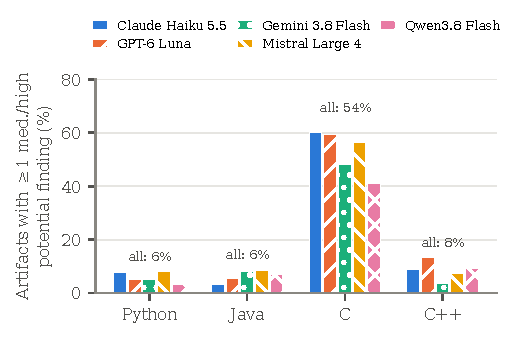
\includegraphics[width=\columnwidth]{figures/fig_security.pdf}
\caption{Share of gate-1-passing artifacts with at least one medium- or
high-severity potential finding, by language. Values in
Table~\ref{tab:seclang}.}
\label{fig:sec}
\end{figure}

\begin{table}[t]
\caption{Artifacts with $\geq$1 medium/high potential finding (\%), by model
and language}
\label{tab:seclang}
\centering\footnotesize
\begin{tabular}{@{}lrrrr@{}}
\toprule
Model & Python & Java & C & C++ \\
\midrule
Claude Haiku 5.5 & 7.7 & 3.2 & 60.0 & 8.7 \\
GPT-6 Luna & 5.0 & 5.4 & 59.3 & 13.3 \\
Gemini 3.8 Flash & 5.1 & 7.9 & 48.0 & 3.5 \\
Mistral Large 4 & 8.1 & 8.6 & 56.5 & 7.4 \\
Qwen3.8 Flash & 3.2 & 6.9 & 41.2 & 9.1 \\
\midrule
All & 5.9 & 6.5 & 53.8 & 8.4 \\
\bottomrule
\end{tabular}

\end{table}

\textbf{Triage of a sample (AI-assisted, unconfirmed).}
\label{sec:triage}
We drew all \nTriageHigh{} high-severity findings and a seeded random sample of
\nTriageMedium{} medium-severity findings on gate-1-passing artifacts, and
classified each from its source context (Table~\ref{tab:triage}). The proposed
labels are \nTriageTP{} likely true positives, \nTriageNC{} that need human or
deployment context, and \nTriageFP{} likely false positives. The likely true
positives are mostly user input reaching a shell in the command-execution task
(CWE-78). The others are AES-CBC with a static initialization vector, which the
task itself mandates, and an unchecked \texttt{atoi} conversion used as an
allocation size (CWE-190). Typical false positives are fixed-size buffers that
are only ever written with bounded functions, \texttt{scanf("\%d")} flagged as
unsafe, \texttt{strcat} into a buffer sized exactly to the result, and a
reported double free on a path that returns before the second free. Of the
\nFlawfinderSampled{} sampled Flawfinder findings, \nFlawfinderFP{} were
labelled likely false positives. These labels are a proposal for human review,
not a measured precision; they indicate that headline scanner counts, ours
included, substantially overstate confirmed weaknesses.

\begin{table}[t]
\caption{AI-proposed triage of \nTriage{} sampled findings (not human-confirmed)}
\label{tab:triage}
\centering\footnotesize
\begin{tabular}{@{}lrrrr@{}}
\toprule
Tool & Likely TP & Needs context & Likely FP & Sampled \\
\midrule
Semgrep & 2 & 1 & 14 & 17 \\
Bandit & 1 & 6 & 0 & 7 \\
Flawfinder & 6 & 10 & 25 & 41 \\
\midrule
All & 9 & 17 & 39 & 65 \\
\bottomrule
\end{tabular}

\end{table}

\subsection{RQ4: Size, Complexity and Reliability}

Tables~\ref{tab:quality} and~\ref{tab:qualitylang} report Lizard and Cppcheck
results on gate-1-passing artifacts. Mistral Large 4 and Qwen3.8 Flash wrote the
shortest code; GPT-6 Luna had the highest mean complexity and the most functions
with CCN above 10. Complexity density is similar across models (mean CCD
\ccdAll{} overall), because longer code also carries more branches. C has the
highest mean CCN for every model. Mistral Large 4 had by far the highest
Cppcheck density (\cppcheckMistral{} findings per C/C++ KLOC, against
\cppcheckLuna{} for GPT-6 Luna). Its findings are almost entirely low-severity
style reports such as \texttt{const}-correctness and STL-algorithm suggestions.
These differences are descriptive; no quality measure was available for Python
or Java beyond size and complexity.

\begin{table}[t]
\caption{Mean NLOC, mean per-artifact CCN, mean CCD, functions with CCN $>$ 10,
and Cppcheck findings per KLOC of C/C++ code (gate-1-passing artifacts)}
\label{tab:quality}
\centering\footnotesize
\setlength{\tabcolsep}{2.5pt}
\begin{tabular}{@{}lrrrrr@{}}
\toprule
Model & NLOC & CCN & CCD & Fn.\ CCN$>$10 & Cppcheck/KLOC \\
\midrule
Claude Haiku 5.5 & 49.9 & 3.41 & 0.336 & 15 & 5.21 \\
GPT-6 Luna & 48.5 & 4.52 & 0.345 & 36 & 3.69 \\
Gemini 3.8 Flash & 56.7 & 3.53 & 0.295 & 15 & 5.56 \\
Mistral Large 4 & 35.6 & 3.29 & 0.315 & 6 & 21.27 \\
Qwen3.8 Flash & 34.8 & 4.07 & 0.343 & 10 & 7.68 \\
\midrule
All & 45.7 & 3.76 & 0.326 & 82 & 7.76 \\
\bottomrule
\end{tabular}

\end{table}

\begin{table}[t]
\caption{Complexity by language (mean CCN / mean CCD) and Cppcheck findings
per KLOC for C and C++}
\label{tab:qualitylang}
\centering\scriptsize
\setlength{\tabcolsep}{2.5pt}
\begin{tabular}{@{}lrrrrrr@{}}
\toprule
 & \multicolumn{4}{c}{Mean CCN / mean CCD} & \multicolumn{2}{c}{Cppcheck/KLOC} \\
\cmidrule(lr){2-5}\cmidrule(l){6-7}
Model & Python & Java & C & C++ & C & C++ \\
\midrule
Claude Haiku 5.5 & 3.09/0.43 & 3.24/0.29 & 4.46/0.30 & 3.05/0.27 & 2.6 & 8.8 \\
GPT-6 Luna & 3.88/0.44 & 3.86/0.30 & 6.46/0.31 & 4.37/0.32 & 1.5 & 5.4 \\
Gemini 3.8 Flash & 2.65/0.36 & 3.25/0.27 & 5.55/0.28 & 3.33/0.25 & 0.6 & 9.8 \\
Mistral Large 4 & 2.61/0.41 & 3.26/0.28 & 4.70/0.29 & 3.04/0.26 & 27.1 & 14.9 \\
Qwen3.8 Flash & 3.21/0.43 & 4.23/0.30 & 6.23/0.33 & 3.30/0.29 & 5.0 & 10.4 \\
\midrule
All & 3.08/0.41 & 3.55/0.29 & 5.46/0.30 & 3.45/0.28 & 6.2 & 9.3 \\
\bottomrule
\end{tabular}

\end{table}

\subsection{RQ5: Cost Versus Quality}

Recorded generation cost for 160 combinations ranged from \$\costLuna{} (GPT-6
Luna) to \$\costMistral{} (Mistral Large 4), a factor of
\costRatioMistralLuna{} (Table~\ref{tab:models}, Fig.~\ref{fig:cost}). Costs
include failed and retried attempts. Cost per 1,000 gate-1-passing artifacts was
\$\costPerPassLuna{} for GPT-6 Luna, \$\costPerPassHaiku{} for Claude Haiku
5.5 and \$\costPerPassMistral{} for Mistral Large 4. The two
cheapest models are not worse: GPT-6 Luna has the highest gate-1 rate, and
potential-finding rates do not differ meaningfully between models. Higher price
therefore bought neither build reliability nor fewer potential findings on this
task set.

\begin{figure}[t]
\centering
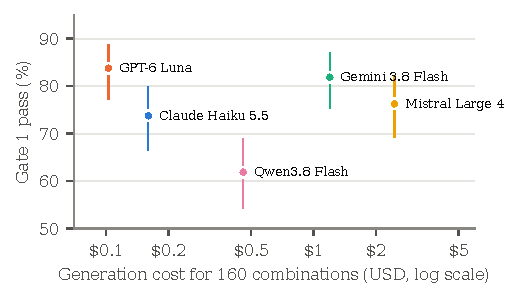
\includegraphics[width=\columnwidth]{figures/fig_cost.pdf}
\caption{Recorded generation cost versus gate 1 pass rate with Wilson 95\%
intervals ($n=160$ per model).}
\label{fig:cost}
\end{figure}

\subsection{Secondary Analysis: Base-Study Outputs}
\label{sec:basecmp}

As a secondary, descriptive analysis we ran our unchanged gate~1 and scanner
pipeline (same flags, tool versions and rule hashes) over the base study's
published C, C++ and Python outputs for the same 40 tasks (\baseNFiles{} files)
\cite{kharma2026}. Java is excluded because no Java outputs were published. The
protocol and its sensitivity analyses were fixed before the run. The
comparison is between \emph{cohorts}, not models. The cohorts differ in models,
prompt, temperature (0.9 in the base study's generation scripts versus
\temperature{}), output-token limits, code extraction and generation date
(2024-era model versions versus ours). The published files are also not pure
model output: \baseNEdited{} of them differ from the copies in the base study's
test repositories, the manual fixes the base study reports cannot be identified
individually, and \baseNEscape{} C/C++ files contain doubled-backslash escapes,
a likely extraction artifact.

Per planned combination, our cohort passed gate~1 less often
(\cohDiffPlanned{}, Table~\ref{tab:basecohort}). The base cohort had more
passing models in \cohCellsBaseHigher{} of \cohCells{} task--language cells and
ours in \cohCellsOursHigher{} (Wilcoxon signed-rank $p$~=~\cohWilcoxonP{}). The gap
comes from our \oursNNoArtifactCCpp{} failed generations and
\oursNIntegrityCCpp{} integrity failures, mostly truncations. Per file with an
artifact, the rates are indistinguishable (\cohDiffArtifact{}). This holds when
escape-pattern files are excluded (\cohDiffArtifactSTwo{}) and in a post-hoc
check that ignores our ledger-only truncation flag, which base files cannot fail
(\cohDiffArtifactSFour{}). It does not hold when only the \baseNIdentical{}
unedited base files are kept (\cohDiffArtifactSOne{}), a subset possibly
selected towards files that needed no fixes. It also fails when blocked files
are removed from the denominator (\cohDiffArtifactSThree{}), because base files
were blocked by missing headers more often (\baseNBlocked{} versus
\oursNBlockedCCpp{}). The per-artifact comparison therefore has no robust
direction.

The share of gate-1-passing files with at least one medium- or high-severity
potential finding does not differ overall (\cohDiffMedHigh{}), nor in the
unedited or escape-free subsets (\cohDiffMedHighSOne{}, \cohDiffMedHighSTwo{}).
It is lower in our Python files (\cohDiffMedHighPy{}). Base files are much
shorter (mean function NLOC \cohNlocBase{} versus \cohNlocOurs{}), so per-file
and per-KLOC rates such as Cppcheck density (\cohCppcheckBase{} versus
\cohCppcheckOurs{} per KLOC, C/C++) are confounded by size. We draw no
model-level or causal conclusion from this comparison, and scanner hits remain
potential findings.

\begin{table}[t]
\centering
\caption{Secondary cohort comparison, ours / base study published outputs (\%,
except NLOC). Same pipeline; C, C++ and Python only; 200 planned combinations
per language and cohort.}
\label{tab:basecohort}
\scriptsize
\begin{tabular}{@{}lrrrr@{}}
\toprule
& Gate 1 / planned & Gate 1 / artifact & $\geq$1 med./high & mean NLOC \\
\midrule
C & 58.5 / 71.0 & 66.9 / 71.0 & 53.8 / 47.9 & 53.7 / 21.2 \\
C++ & 65.5 / 71.0 & 71.6 / 71.0 & 8.4 / 10.6 & 48.4 / 17.4 \\
Python & 93.0 / 99.0 & 99.5 / 99.0 & 5.9 / 13.1 & 36.1 / 7.0 \\
\midrule
All & 72.3 / 80.3 & 79.6 / 80.3 & 19.6 / 22.6 & 44.5 / 14.3 \\
\bottomrule
\end{tabular}

\end{table}

%==========================================================================
\section{Discussion}
%==========================================================================

\textbf{Language matters more than model.} Across all three measurements, the
spread between languages exceeds the spread between models. C combines the
lowest build rate with the highest rate of potential findings, which agrees with
the base study \cite{kharma2026}. Much of the C/C++ build loss is truncation at
the output limit and missing third-party headers rather than syntax errors. A
larger output budget, or tasks that avoid third-party libraries, would change
these numbers more than the choice of model would.

\textbf{Failure modes differ by model.} Qwen3.8 Flash mostly failed by emitting
nothing within the token budget, Claude Haiku 5.5 by truncation, and Gemini 3.8
Flash and Mistral Large 4 by refusing one malware-like task. These are distinct
operational risks, and a single pass rate hides them.

\textbf{Reusing published tests is harder than it looks.} Only
\nOracleApproved{} of \nOracleProposed{} proposed reference tests survived
review, and the survivors cover mostly simple algorithmic tasks on which every
model succeeded. Benchmarks that ship tests written against one model's
implementation measure agreement with that implementation, not with the task.
We recommend that future datasets ship language-specific tests written against
a fixed, documented interface, together with the task.

\textbf{Scanner counts are not vulnerability counts.} The AI-assisted triage
labelled most sampled findings as likely false positives. This is consistent
with prior evidence that static verdicts diverge from human judgement
\cite{tessa2026,firouzi2026}. We therefore report potential-finding rates with
intervals, keep each tool separate, and make no claim about confirmed
vulnerability rates.

\textbf{Direction for future work.} The likely true positives cluster where a
task requires a dangerous capability, such as executing a user command or
using a fixed IV. The weakness there sits at a specific enforcement point. This
motivates approaches that bind security obligations to named locations in the
code and validate the corresponding tests against weakened variants. We
outlined such a design (``ContractGuard'') during this project, but it was not
implemented or evaluated and no result in this paper concerns it.

%==========================================================================
\section{Threats to Validity}
%==========================================================================

\textbf{Construct validity.} Gate 1 shows that code is complete and compiles,
not that it is correct. Python imports are not resolved, and C/C++ are compiled
without linking. Static scanners measure potential issues, and our triage
labels are AI-assisted proposals that have not been human-confirmed. The
oracle and adapter decisions that determine functional coverage were also made
with AI assistance and need human confirmation; Section~\ref{sec:audit} gives
the criteria, and every decision is recorded with its reason. NLOC counts
only code inside functions, so per-KLOC rates are approximate for script-style
artifacts. The functional pass rate is conditional on testability and saturated.
It must not be compared with rates over all \nPlanned{} combinations.

\textbf{Internal validity.} The generation prompt is ours, not the base study's.
Temperature \temperature{} with one sample per combination does not capture
sampling variance. Retries on empty or invalid responses favour models that
recover. Gate 1 uses clang for C/C++ while functional builds use gcc; a build
difference would surface as an error, not a failure. A first functional run
contained harness defects (a verdict bug and a missing import in the Java
facade). It was superseded after the defects were fixed and regression tests
added, and all reported functional results come from the second run.

\textbf{External validity.} Forty tasks were chosen by judgment within strata,
not randomly. Each cell of model and language has 40 tasks, so per-cell
intervals are wide. The models are cost-efficient tiers; results may not
transfer to flagship models, to agentic workflows, or to repository-scale code.
A pilot of \pilotPlanned{} further combinations (10 disjoint tasks, all from the
security strata), generated by the same five models with identical settings and
used to validate the runner, was evaluated separately with the same gate~1 and scanners and is not
pooled with the main results. Its language pattern matches: gate~1 pass rates
of \pilotGOnePy{} (Python), \pilotGOneJava{} (Java), \pilotGOneCpp{} (C++) and
\pilotGOneC{} (C), \pilotGOnePass{} overall, and C again has the highest share
of passing artifacts with a medium- or high-severity potential finding
(\pilotMedHighC{}).
Model identifiers are as listed in Table~\ref{tab:modelids}; providers may
update models behind an identifier. The comparison with the base study's
outputs (Section~\ref{sec:basecmp}) is confounded by the generation protocol and
by post-processing of the published files, and supports no model-level claim.

\textbf{Reliability.} All numbers in this paper are generated from the released
per-combination results by a script, and a separate script recomputes the quality
and paired statistics from raw tool output, checking the statistics against SciPy.
The raw ledgers, artifact hashes, scanner versions and rule-pack hashes are
recorded. An earlier consolidation divided Cppcheck findings by the lines of
all four languages, understating C/C++ density about twofold; all values here
use C/C++ lines only. CodeQL and SonarQube, which the base
study used, were not run.

%==========================================================================
\section{Conclusion}
%==========================================================================

We measured five current cost-efficient LLMs on \nPlanned{} task, model and
language combinations derived from a published multi-language study, keeping
confirmed checks, executed tests, potential scanner findings, and untested
combinations apart. Three quarters of combinations produced complete,
compilable code. The language effect clearly exceeded the model effect, with C
weakest on both build rate and potential findings, and the most expensive model
was no better than the cheapest. Functional tests recovered from the original
study proved largely unusable as they were, and the executable remainder was
too easy to separate the models. Scanner findings were frequent in C but, in an
unconfirmed triage, mostly false positives. The two most useful next steps are
human confirmation of the oracle, adapter and triage decisions, and
interface-fixed functional and security tests for the security-relevant tasks,
so that correctness and exploitability can be measured where they matter most.

\section*{Data Availability}
The generation runner, evaluation pipeline, sandbox scripts, per-combination
results, review decisions with reasons, and the scripts that generate every
number and figure in this paper are available in the project repository. The
recovered upstream tests are not redistributed because their repositories
declare no license; they are fetched at pinned commits.
% TODO (authors): add the repository URL once it is public.

\section*{Acknowledgment}
% TODO (authors).

%==========================================================================
\begin{thebibliography}{00}

\bibitem{kharma2026} M. F. Kharma, S. Choi, M. Alkhanafseh, and D. Mohaisen,
``Security and quality in LLM-generated code: A multi-language, multi-model
analysis,'' \textit{IEEE Trans. Dependable Secure Comput.}, vol.~23, no.~3,
pp.~7300--7314, May/Jun. 2026, doi: 10.1109/TDSC.2026.3672745.

\bibitem{securecoder2025} J. Zhao, Y. Sun, C. Huang, C. Liu, Y. Guan, Y. Zeng,
and Y. Liu, ``Towards secure code generation with LLMs: A study on Common
Weakness Enumeration,'' \textit{IEEE Trans. Softw. Eng.}, vol.~51, no.~12,
pp.~3507--3523, Dec. 2025.

\bibitem{perry2023} N. Perry, M. Srivastava, D. Kumar, and D. Boneh, ``Do users
write more insecure code with AI assistants?'' in \textit{Proc. ACM SIGSAC Conf.
Comput. Commun. Secur. (CCS)}, 2023, arXiv:2211.03622.

\bibitem{metr2025} J. Becker, N. Rush, E. Barnes, and D. Rein, ``Measuring the
impact of early-2025 AI on experienced open-source developer productivity,''
2025, arXiv:2507.09089.

\bibitem{baxbench2025} M. Vero, N. M\"undler, V. Chibotaru, V. Raychev
\textit{et al.}, ``BaxBench: Can LLMs generate correct and secure backends?''
2025, arXiv:2502.11844.

\bibitem{susvibes2026} S. Zhao, D. Wang, K. Zhang, J. Luo \textit{et al.}, ``Is
vibe coding safe? Benchmarking vulnerability of agent-generated code in
real-world tasks,'' 2025, arXiv:2512.03262.

\bibitem{cweval2025} J. Peng, L. Cui, K. Huang, J. Yang \textit{et al.},
``CWEval: Outcome-driven evaluation on functionality and security of LLM code
generation,'' 2025, arXiv:2501.08200.

\bibitem{mtsec2025} R. Rawal, J. Y. F. Chiang, C. Shen, J. S. Tian \textit{et
al.}, ``Benchmarking correctness and security in multi-turn code generation,''
2025, arXiv:2510.13859.

\bibitem{tessa2026} M. Tessa, I. E. Olatunji, A. War, J. Klein \textit{et al.},
``How secure is secure code generation? Adversarial prompts put LLM defenses to
the test,'' 2026, arXiv:2601.07084.

\bibitem{firouzi2026} E. Firouzi and M. Ghafari, ``Persistent human feedback,
LLMs, and static analyzers for secure code generation and vulnerability
detection,'' 2026, arXiv:2602.05868.

\bibitem{sok2026} R. Patir, K. Guo, H. Cai, and H. Hu, ``SoK: AI secure code
generation: Progress, pitfalls, and paths forward,'' 2026, arXiv:2606.25195.

\bibitem{dai2025} S.-C. Dai, J. Xu, and G. Tao, ``Rethinking the evaluation of
secure code generation,'' 2025, arXiv:2503.15554.

\bibitem{scaffold2026} Y. Chen, Y. Bian, H. Wang, S. Li \textit{et al.},
``SCAFFOLD-CEGIS: Preventing latent security degradation in LLM-driven
iterative code refinement,'' 2026, arXiv:2603.08520.

\bibitem{macot2026} M. F. Kharma, M. Alkhanafseh, A. Sabbah, and D. Mohaisen,
``Enhancing reliability in LLM-based secure code generation,'' 2026,
arXiv:2605.24300.

\bibitem{csdd2026} S. R. Marri, ``Constitutional spec-driven development:
Enforcing security by construction in AI-assisted code generation,'' 2026,
arXiv:2602.02584.

\bibitem{specdriven2026} O. Grynets, A. Salyk, V. Lyashkevych, O. Kaskun
\textit{et al.}, ``Specification-driven development benchmark: Security
knowledge transition,'' 2026, arXiv:2606.00167.

\bibitem{wilson1927} E. B. Wilson, ``Probable inference, the law of succession,
and statistical inference,'' \textit{J. Amer. Statist. Assoc.}, vol.~22,
no.~158, pp.~209--212, 1927.

\bibitem{mcnemar1947} Q. McNemar, ``Note on the sampling error of the difference
between correlated proportions or percentages,'' \textit{Psychometrika},
vol.~12, no.~2, pp.~153--157, 1947.

\bibitem{holm1979} S. Holm, ``A simple sequentially rejective multiple test
procedure,'' \textit{Scand. J. Statist.}, vol.~6, no.~2, pp.~65--70, 1979.

\bibitem{newcombe1998} R. G. Newcombe, ``Improved confidence intervals for the
difference between binomial proportions based on paired data,''
\textit{Statist. Med.}, vol.~17, no.~22, pp.~2635--2650, 1998.

\bibitem{semgrep} Semgrep, Inc., ``Semgrep,'' [Online]. Available:
\url{https://github.com/semgrep/semgrep}

\bibitem{bandit} PyCQA, ``Bandit,'' [Online]. Available:
\url{https://github.com/PyCQA/bandit}

\bibitem{flawfinder} D. A. Wheeler, ``Flawfinder,'' [Online]. Available:
\url{https://dwheeler.com/flawfinder/}

\bibitem{cppcheck} ``Cppcheck: A tool for static C/C++ code analysis,''
[Online]. Available: \url{https://cppcheck.sourceforge.io/}

\bibitem{lizard} T. Yin, ``Lizard: A simple code complexity analyser,''
[Online]. Available: \url{https://github.com/terryyin/lizard}

\bibitem{bubblewrap} ``Bubblewrap: Low-level unprivileged sandboxing tool,''
[Online]. Available: \url{https://github.com/containers/bubblewrap}

\end{thebibliography}

\end{document}
